
\chapter{Paginazione}
Tradurre gli indirizzi virtuali in indirizzi fisici singolarmente è una cosa veramente improponibile. 
\paragraph{Cosa facciamo?}
\begin{itemize}
	\item Dividiamo lo spazio di indirizzamento virtuale in regioni naturali dette \emph{pagine}.
	\item Dividiamo lo spazio di indirizzamento fisico in regioni naturali dette \emph{frame}.
\end{itemize}
Pagine e frame hanno la stessa dimensione: $4\,\text{KiB}$ (0x1000 in esadecimale). La pagina viene inserita in un frame e si identifica perfettamente con esso: non esiste una pagina posta tra frame diversi.
\paragraph{Traduzione degli indirizzi in una pagina} Tutti gli indirizzi posti in una pagina sono tradotti in maniera contigua (la traduzione effettiva avviene nei bit più significativi, non nell'offset).
%\begin{center}
%	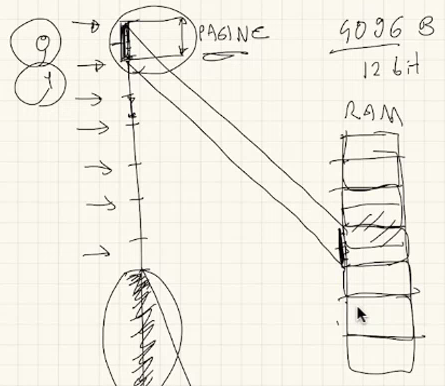
\includegraphics[scale=.8]{img/212.PNG}
%\end{center}
\section{\emph{Memory Management Unit} (MMU)}
Abbiamo introdotto l'organizzazione in pagine, ma non abbiamo ancora detto come gestiremo il passaggio da indirizzo virtuale a indirizzo fisico, tenendo conto che la traduzione dovrà essere diversa per ogni pagina. Introduciamo l'\textbf{unità di gestione della memoria} tra CPU e Cache.
\begin{itemize}
	\item Si osservi che la MMU non ha un buco come lo spazio di indirizzamento: negli indirizzi presenti si ha un salto dall'ultimo indirizzo prima del buco al primo indirizzo dopo il buco.
	\item La cache fa parte del mondo fisico, può ignorare l'introduzione della \emph{Memory Management Unit} (MMU). La MMU traduce gli indirizzi virtuali in base alla traduzione attiva in un certo istante: la struttura dati utilizzata dalla MMU può essere immaginata come un insieme di \textit{tabelle di corrispondenza} (una per processo). Queste tabelle sono un esempio di struttura dati condivisa tra hardware e software: quest'ultimo (il kernel) stabilisce quali tabelle ci sono e quali sono attive.
\end{itemize}
\begin{center}
	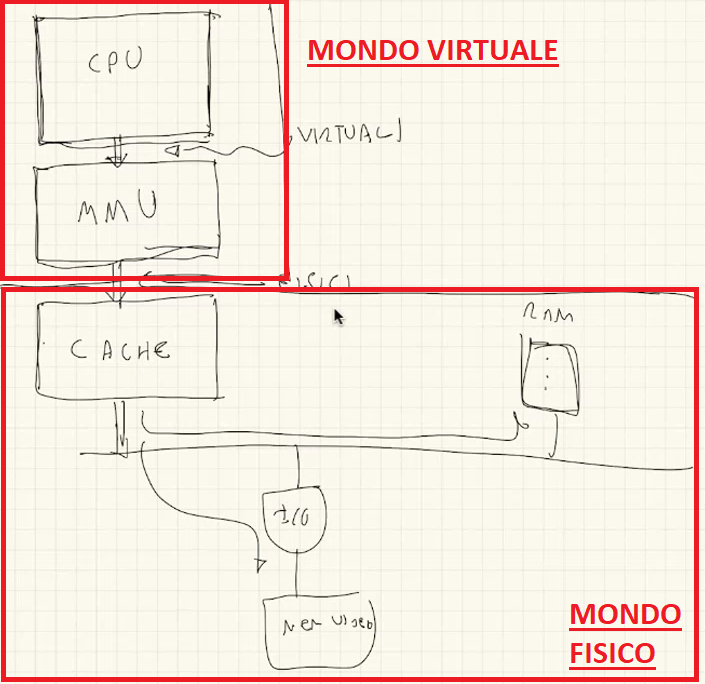
\includegraphics[scale=.5]{img/213.PNG}
\end{center}

\subsection{Passaggio da indirizzo virtuale a indirizzo fisico} 
\begin{center}
	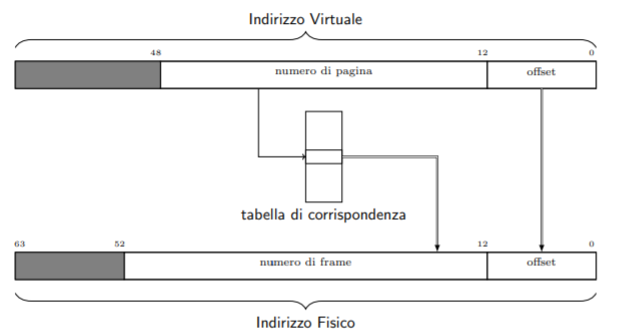
\includegraphics[scale=.9]{img/214.PNG}
\end{center}
\begin{itemize}
	\item Nell'indirizzo indicato dalla CPU si distingue l'\emph{offset} (bit meno significativi) dal \emph{numero di pagina} (bit più significativi).
	\item Il numero di pagina va in ingresso nella tabella di corrispondenza relativa al processo: l'indice posto in ingresso mi restituisce il corrispondente  \emph{numero di frame}. 
	\item Ogni tabella di corrispondenza ha una riga per ogni possibile pagina (non poche, visto il numero di bit riservati al numero di pagina). 
\end{itemize}
\paragraph{Attenzione al numero di bit} Gli indirizzi fisici fanno riferimento allo spazio di indirizzamento fisico, quelli virtuali allo spazio di indirizzamento virtuale. Il numero di bit massimo è $64$, varie generazioni di CPU implementano indirizzi virtuali su un numero inferiore di bit. La questione dipende dal modello della CPU, tutto lì (cit.). 

\subsection{Contenuto delle tabelle di corrispondenza} Ciascuna riga delle tabelle di corrispondenze è grande 8 byte: il numero di frame si trova nella posizione in cui si troverebbe all'interno dell'indirizzo (per comodità del programmatore, in questo caso si va dal bit 12 al bit 52). Le righe non contengono solo il corrispondente \emph{numero di frame}, ma anche una serie di flag (di cui non ci interessa la posizione):
\begin{itemize}
	\item un flag $U/S$ che mi indica se la pagina può essere acceduta solo a livello utente o anche a livello sistema (quindi distinguo attraverso questo flag i frame relativi all'area riservata al livello sistema dai rimanenti\footnote{Viene meno la necessità di un registro che indica l'indirizzo limite tra area riservata al sistema e il resto.});
	\item un flag $R/W$ che mi indica se la scrittura nella pagina è permessa o no;
	\item un flag $P$ (presenza) che mi dice se la traduzione è valida (quindi se l'indirizzo corrisponde, al di la del livello di privilegio). Si utilizza per marcare le pagine che il processo non usa (che avranno $P=0$);
	\begin{itemize}
		\item Il flag $P$ può essere utilizzato per vietare l'utilizzo dell'indirizzo $0$ (mi basta porre $0$ nella pagina relativa). Nel caso di accesso a una pagina con $P=0$ il processore solleva un'eccezione \emph{page fault} (fault perchè il sistema potrebbe aggiustare lo stato della memoria e rieseguire l'istruzione attraverso la \emph{paginazione su domanda}, che vedremo a Sistemi Operativi\footnote{Uno dei pochi esempi di \emph{fault} effettivamente risolti}).
	\end{itemize}
	\item i flag PWT (\emph{Page Write Through}) e PCD (\emph{Page Cache Disable}), con cui la MMU trasmette dei comandi alla cache (il secondo ordina alla cache di non intercettare l'operazione, il primo chiede di utilizzare alla cache di usare la politica \emph{write-through}).
	\begin{itemize}
		\item Il flag PCD è utile per tutte le pagine che contengono indirizzi di registri di I/O mappati in memoria, invece che locazioni di memoria (per esempio l'APIC). 
		\item Il flag PWT è utile per quanto riguarda la parte di indirizzi relativa alla memoria video: vogliamo che la scrittura vera arrivi nella memoria video, e che non rimanga in cache.
	\end{itemize}
\end{itemize}


\paragraph{Flag per la paginazione su domanda} Abbiamo i bit $A$ e $D$ che sono legati all'implementazione della paginazione su domanda. La MMU setta il bit $A$ di una entrata quando la MMU accede alla relativa entrata per fare una traduzione, mentre setta il bit $D$ se l'accesso all'indirizzo relativo alla pagina era in scrittura.
\paragraph{Bit NX} Ulteriore bit è il \emph{Not executable}. Se durante l'operazione di fetch di un'istruzione abbiamo $NX=1$ per la relativa pagina allora il processore genera un'eccezione.





%I processi non ci dicono l'indirizzo di memoria RAM a cui vogliono accedere, ma solo l'offset. A runtime il registro LINF non viene usato come limite, ma per essere sommato all'offset.
%- Lo spazio di indirizzamento del processore presenta, oltre alla RAM, periferiche: APIC, memoria video in modalità grafica, memoria video in modalità testo (che nasconde parte della RAM), abbiamo parlato di \emph{Memory Mapped I/O}. La cosa è problematica per la \emph{Cache}, che normalmente lavora solo con lo spazio di memoria. Vogliamo disattivarla, l'unica cosa che può distinguere due operazioni è l'indirizzo. La soluzione è limitare l'accesso alle periferiche sulla base degli indirizzi, e non dell'istruzione eseguita.

%Protezione:
%Negli accessi in memoria la cosa è più sofisticata rispetto a dire livello utente o livello sistema (cosa che comunque è presente).
%- Nella parte dedicata all'utente c'è un qualcosa di più: pensiamo ai programmi, che possono essere letti ma non sovrascritti.
%- Il \textit{null pointer} è rappresentato con l'indirizzo 0, quindi quell'indirizzo non può essere utilizzato. Addirittura è possibile stabilire l'inaccessibilità dell'indirizzo pure in modalità sistema. 

\section{MMU e modulo sistema} 
Facciamoci una domanda: siamo obbligati a mappare gli indirizzi relativi al modulo sistema nello spazio di indirizzamento virtuale dei vari processi? Sì: se siamo a livello utente e sollevo un'eccezione la CPU inizia a fare un po' di cose, come consultare l'IDT e il TSS, o scrivere dentro la pila sistema. Tutti questi indirizzi saranno tradotti dalla MMU, dunque in assenza di mapping la gestione delle interruzioni non è possibile

\paragraph{Cosa faremo} La cosa più semplice è mappare tutta la memoria di sistema: quando siamo a livello utente e avviene un passaggio a livello sistema la CPU troverà tutto ciò che le serve (visto che tutto è mappato). In questa parte di indirizzamento mapperemo tutta la zona di RAM che contiene il codice e le strutture dati presenti nel modulo sistema. Cosa importante
\[\boxed{\text{Tutto è mappato agli stessi indirizzi in ogni processo}}\]
\paragraph{Tabelle di corrispondenza e cambio di processo} Se il sistema vuole fare un cambio di processo allora deve cambiare la tabella di corrispondenza. Se non facciamo ciò l'\textit{Instruction pointer} va avanti interpretando gli indirizzi in modo inaspettate (traduco col contenuto della tabella di corrispondenza del vecchio processo, non con quella del processo in esecuzione).

\paragraph{Aspetto complicato} Scrivere codice sistema essendo costantemente consapevoli della differenza tra indirizzi fisici e indirizzi virtuali. Lavorando a livello utente questo ignora che i suoi indirizzi sono virtuali: gli utenti usano solo questi e non hanno interesse sugli indirizzi fisici.

\section{Esempio: indirizzi virtuali e fisici in un programma in esecuzione} 
Scriviamo un programma dove dichiariamo una variabile e ne stampiamo l'indirizzo
\begin{verbatim}
	#include <iostream>
	
	int var;
	int main() {
		std::cout << "&var: "<< &var << "\n";
	}
\end{verbatim}
Compiliamo
\begin{verbatim}
	g++ -o myprog.cc -no-pie myprog.cc
	./myprog
\end{verbatim} 
Otteniamo
\begin{verbatim}
	&var: 0x404174
\end{verbatim}
L'indirizzo stampato è l'indirizzo scelto dal collegatore: compilatore, collegatore e programmatore sono consapevoli solo dell'esistenza di questo indirizzo virtuale (per noi è l'unico indirizzo vero).
\paragraph{Chiediamo l'indirizzo fisico} Se abbiamo livelli di privilegio sufficienti possiamo chiedere l'indirizzo fisico invece di quello virtuale. Modifichiamo il programma per mantenerlo in vita
\begin{verbatim}
	#include <iostream>
	
	int var;
	int main() {
		std::cout << "&var: "<< &var << "\n";
		
		for(;;) {
			sleep(1);
		}
	}
\end{verbatim}
dove \emph{sleep} è l'equivalente unix della \emph{delay}, col numerino che esprime i secondi. Eseguiamo il programma e mentre questo cicla chiediamo col terminale il processor identifier
\begin{verbatim}
	pgrep myprog
\end{verbatim}
successivamente eseguiamo la seguente istruzione
\begin{verbatim}
	sudo ./virt_to_phys 1922 0x404174 // verra' richiesta la password
\end{verbatim}
otteniamo l'indirizzo fisico \textbf{0x49512174}, completamente diverso dall'indirizzo virtuale (tranne che nell'offset, le tre cifre esadecimali meno significative costituiscono l'offset all'interno della pagina).
\begin{itemize}
	\item La variabile var si trova nella pagina 404 all'offset 174.
	\item La MMU trasforma il numero di pagina nel numero di frame 495121, non l'offset.
\end{itemize}
Proviamo ad eseguire un'altra istanza del programma, senza chiudere la precedente. Con le stesse cose fatte prima otteniamo l'indirizzo fisico \textbf{0x4ed18174}: non è cambiato l'offset (174), ma è cambiato il numero di frame (4ed18). Ognuno vive nel suo mondo senza conoscere l'esistenza dell'altro.

\section{MMU all'opera}
\small
Nelle diapositive seguenti viene spiegato nel dettaglio il comportamento della MMU con le sue \emph{tabelle di corrispondenza}. 
\begin{itemize}
	\item Viene introdotto un programma in C++ che agisce su uno spazio di indirizzamento virtuale. Si suppone, per ragioni di semplicità, che lo spazio di indirizzamento virtuale sia di $32\,\text{KiB}$ (gli indirizzi vanno da 0000 a 7fff).
	\item Lo spazio di indirizzamento viene diviso in 8 pagine, ciascuna da $4\,\text{KiB}$ (nulla di nuovo).
	\item Le pagine $0$ e $1$ sono riservate al sistema.
	\item La pagina $2$ contiene il codice del programma (da 2000 a 2fff).
	\item Le pagine $3$ e $4$ contengono la variabile \emph{buf}.
	\item La pagina $7$ viene usata come pila.
\end{itemize}
Successivamente viene introdotto un secondo processo, più piccolo. Le diapositive mostrano come la MMU operi con due processi.
\normalsize 

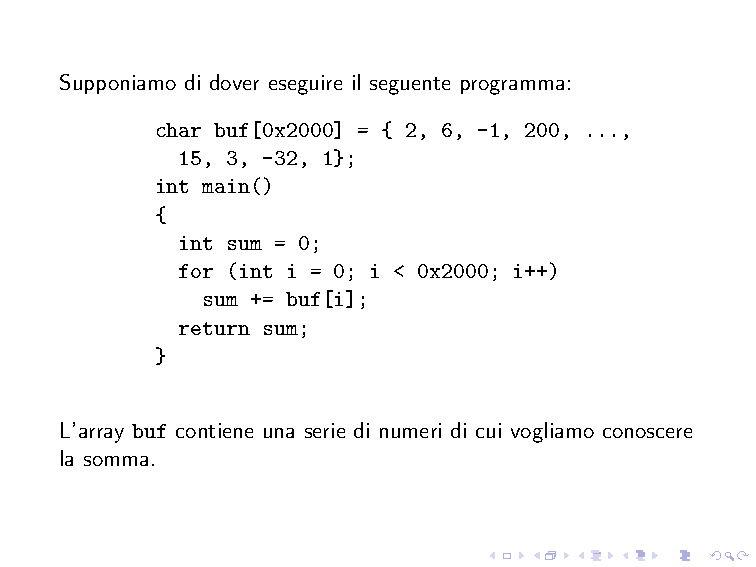
\includepdf[pagecommand={\thispagestyle{plain}},frame,scale=0.93,frame,nup=2x3,pages=-]{pdf/supermmu}

\section{Tabelle di corrispondenza multilivello (\emph{bitwise trie})}
\paragraph{Quanto è grande una tabella di corrispondenza?} Supponiamo di avere uno spazio di $2^{48}$ byte: considerato che ogni pagina è grande $2^{12}$ byte otteniamo il seguente numero di pagine
\[\frac{2^{48}}{2^{12}}=2^{36}\]
La dimensione di ogni entrata è di 8 byte: segue la dimensione della tabella di corrispondenza
\[2^{36} \times 8\,\text{byte}=512\,\text{GiB}\]
Morale della favola: è difficile avere un dispositivo che mi possa contenere una sola di queste tabelle. Ci serve una struttura dati che mi permetta di associare una chiave a un valore
\[\boxed{\text{Chiave (Numero di pagina)} \longrightarrow \text{Valore (Numero di frame)}}\]
\paragraph{Struttura dati} La struttura dati immaginata è una variante del \emph{trie}
: il \emph{bitwise trie}. Con \emph{trie} intendiamo strutture dati ad albero con cui mappiamo chiavi di tipo stringa. Supponiamo di avere le seguenti associazioni
\[\begin{array}{l}\text{trip} \longrightarrow \text{viaggio}\\\text{tree} \longrightarrow \text{albero}\\\text{hill} \longrightarrow \text{collina}\\\text{hot} \longrightarrow \text{caldo}\\\text{house} \longrightarrow \text{casa} \end{array}\]
Otteniamo il seguente albero:
\begin{center}
	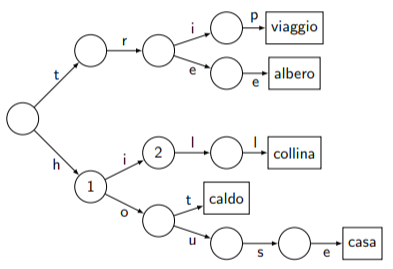
\includegraphics{img/215.PNG}
\end{center}
\begin{itemize}
	\item I caratteri guidano i nostri movimenti all'interno dell'albero: gli archi sono marcati con i caratteri delle chiavi e il valore associato ad ogni chiave si trova nella foglia che si raggiunge partendo dalla radice e seguendo il percorso indicato dalla chiave. 
	\item L'inserimento di una nuova associazione chiave-valore comporta una visita nell'albero come in una ricerca, con la creazione di eventuali nodi mancanti fino alla foglia che deve contenere il valore.
\end{itemize}
Tenendo conto che il trie si basa sulla codifica ASCII possiamo immaginarci un'implementazione dove ogni nodo consiste in un array di 128 entrate: ogni elemento dell'array è nullo o contiene un puntatore ad un altro nodo (quindi ad un altro array).

\paragraph{\emph{bitwise trie}} Il bitwise trie è una variante che prevede al posto dei caratteri gruppi di bit della chiave. L'indirizzo della radice è posto nel registro \emph{CR3} della MMU.
\begin{itemize}
	\item Il numero di pagina è composto da 36 bit, che raggruppiamo in quattro gruppi da 9 bit ciascuno. Nello scorrimento dell'albero consideriamo i gruppi \textbf{da quelli con le cifre più significative a quelli con le meno significative}.
	\item Ogni nodo del bitwise trie risulterà essere una tabella di $2^9=512$ entrate. Ciascuna entrata è un puntatore che può essere nullo, o rimandare a un nodo successivo.
	\item Sappiamo che ogni entrata ha dimensione di 8 byte, dunque otteniamo che ogni tabella ha dimensione
	\[512 \cdot 8\,\text{byte}=4096\,\text{byte}\]
	\item L'albero ha al più 4 livelli, numerati dalla radice in senso decrescente (da $4$ ad $1$)
	\begin{center}
		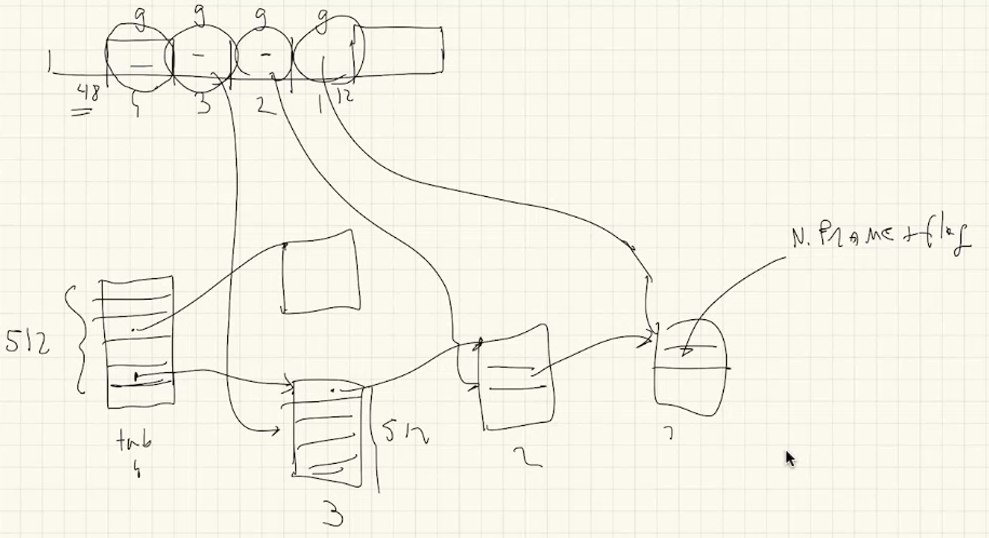
\includegraphics[scale=.55]{img/216.PNG}
	\end{center}
	Se noi mettiamo insieme tutti i nodi, tutte le tabelle, otteniamo la tabella iniziale, ma a dimensione maggiore. Cio è valido solo se realizziamo tutti i sotto-alberi possibili (non abbiamo alberi dove il processo non ha mappato niente). 
	\item Le foglie hanno la stessa struttura dei nodi, l'unica differenza sta nel significato delle entrate (che contengono non un puntatore, ma il numero di frame). 
	\item Ogni riga delle tabelle ha la stessa struttura. Differenza rispetto alle tabelle viste all'inizio introducendo la MMU è la presenza di un maggior numero di bit: questo a causa dell'allineamento naturale delle tabelle (4096 byte), che impone i primi 12 bit meno significativi dell'indirizzo di una tabella uguali a zero. Alcuni bit non sono presenti (per esempio D), mentre altri sono presenti ma hanno un significato radicalmente diverso.
	\item il \emph{page fault} viene generato non appena si individua una riga con $P=0$.
	\item \textbf{Regola per le scritture}. La scrittura è permessa solo se è permessa da tutti i livelli.
	\item \textbf{Regola per l'accesso da livello utente}. L'accesso a livello utente è consentito solo se consentito da tutti i livelli.
\end{itemize}
\begin{framed}
	\noindent \textbf{Recap}
	\begin{itemize}
		\item Abbiamo definito un architettura con la MMU posta tra CPU e Cache, distinguendo un "mondo fisico" con indirizzi fisici da un "mondo virtuale" con indirizzi virtuali (CPU e la MMU, dunque il software).
		\item La MMU, in ogni istante, avrà una traduzione attiva: un albero trie con cui associo un indirizzo fisico a un indirizzo virtuale (ottengo l'indirizzo fisico sostituendo, nell'indirizzo virtuale, il numero di pagina col numero di frame). La CPU contiene un registro, detto CR3, col numero di frame dove si trova la radice dell'albero attivo (l'albero si trova nella RAM, attenzione).
		\item Percorro l'albero utilizzando le varie parti che caratterizzano il numero di pagina: nella foglia troverà il numero di frame. Ricordiamoci che oltre al numero di frame abbiamo altre informazioni associate al numero di pagina.
		\item La struttura ci permette di evitare di associare un frame a qualunque pagina: dove non si può andare l'albero non prosegue, con $P=0$.
	\end{itemize}   
\end{framed}
\paragraph{Domanda sugli indirizzi della struttura dati} Questa è una struttura dati preparata dal sistema e utilizzata dall'hardware (MMU). Nelle varie tabelle sono presenti puntatori ad altre tabelle nella RAM. Ci siamo chiesti: questi puntatori sono indirizzi virtuali o fisici? 
\begin{itemize}
	\item Fisici, altrimenti si genererebbe una sorta di loop (come faccio a muovermi tra le varie tabelle-nodo se ogni puntatore deve essere a sua volta tradotto attraverso le tabelle stesse?). \textbf{Emerge il problema di gestire questi passaggi}.
\end{itemize}

\paragraph{Come fa il software ad accedere a qualunque cosa?} Per accedere a una qualunque entità abbiamo bisogno delle seguenti cose:
\begin{enumerate}
	\item un indirizzo fisico per l'entità;
	\item un indirizzo virtuale associato all'indirizzo fisico dell'entità;
	\item la conoscenza da parte del software dell'indirizzo virtuale (all'utente non serve conoscere l'indirizzo fisico, il software lavora solo con indirizzi virtuali)
\end{enumerate} 

\subsection{Utente e indirizzi virtuali e fisici}
Per l'utente la vita è facile: conosce solo l'indirizzo virtuale. In un programma utente si dichiara una variabile globale, e il collegato sceglie un indirizzo virtuale per questa variabile. La variabile acquisisce un indirizzo fisico perchè il sistema caricherà la sezione data in una pagina, quindi in qualche frame. Il sistema, interpretando il file ELF, vedrà che il collegatore voleva he quella variabile si trovasse a un certo indirizzo virtuale: si crea così una corrispondenza tra indirizzo fisico e indirizzo virtuale.


\paragraph{stack} Per quanto riguarda lo stack non ci sono problemi: creiamo la corrispondenza tra indirizzo fisico e indirizzo virtuale, a quel punto rendo conoscibile  l'indirizzo virtuale mettendolo  nel registro RSP.



\subsection{Sistemi e indirizzi virtuali e fisici}
Per il sistema le cose sono più difficili: deve essere consapevole in modo costante della differenza tra indirizzi fisici e indirizzi virtuali. In alcune situazioni gli indirizzi fisici sono irrinunciabili: le comunicazioni col bus mastering, l'aggiornamento delle tabelle di corrispondenza. Per memorizzare l'albero ci servono dei frame
\begin{center}
	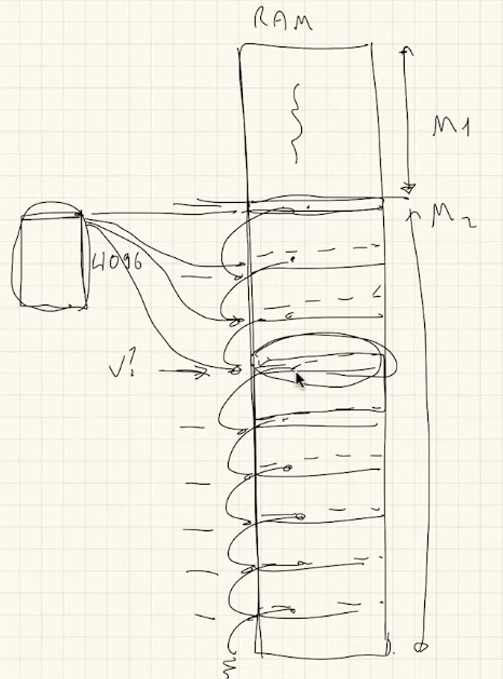
\includegraphics[scale=.7]{img/217.PNG}
\end{center}
in ciascun frame si ha, immaginiamo, un puntatore al frame successivo. Risulta immediato che dobbiamo sistemare qualcosa per poter inizializzare questa lista via software (devo scrivere in indirizzi fisici, mi servirebbe un indirizzo virtuale, ma come faccio se la corrispondenza si ottiene attraverso la tabella che stiamo inizializzando?)

\paragraph{Soluzione} Prendiamo lo spazio di indirizzamento di un qualunque processo e lo dividiamo a metà. 
\begin{itemize}
	\item Una delle due metà viene riservata al sistema (in modo tale che guardando i bit più significativi gli indirizzi siano riconoscibili). Nel nostro caso l'utente andrà a considerare, per le sue cose, solo gli indirizzi che iniziano con $111111$ (cifre più significative).
	\item Ci rimangono indirizzi virtuali a disposizione del sistema: l'idea è di mapparli in tutta la RAM, per fare in modo che tutti gli indirizzi fisici della RAM abbiano un corrispondente indirizzo virtuale, a priori. Questa cosa permetterà al sistema di accedere a tutta la memoria fisica. In contemporanea dobbiamo negare questa possibilità ai processi utente.
	\[\boxed{\text{A questo punto ogni indirizzo fisico ha un corrispondente indirizzo virtuale}}\]
	\item \textbf{Come garantiamo al sistema la conoscenza degli indirizzi virtuali?} Ponendo il numero di frame uguale al numero di pagina, cioè poniamo indirizzi virtuali uguali ad indirizzi fisici! A un certo punto modificheremo CR3: a quel punto la MMU inizierà ad usare un nuovo albero di traduzione. Se vogliamo garantire continuità nel passaggio da un processo a un altro dobbiamo fare in modo che la traduzione degli indirizzi relativi all'area per il sistema siano uguali in entrambi gli alberi. Questa cosa semplifica l'inizializzazione del sistema: la paginazione inizialmente è disattivata, fino a quando non modificheremo un flag nel registro CR0. 
\end{itemize} 

\paragraph{Sorpresa} 
\[\boxed{\text{Fino ad ora abbiamo sempre lavorato con la paginazione attiva}}\]
\noindent La AMD, per come ha realizzato il processore, ha fatto in modo che la modalità  a 64 bit sia in realtà una sotto-modalità della paginazione. Al momento dell'avvio il bootstrap parte come un 8086, viene portato a 32 bit abilitando la protezione, e infine si passa a 64 bit con l'attivazione della paginazione
\[\text{8086 a 16 bit} \longrightarrow \text{32 bit con abilitaz. protezione} \longrightarrow \text{64 bit con abilitaz. paginazione}\]
Questi passaggi avvengono attraverso la modifica di appositi flag.
\paragraph{Registri} Nel processore sono presenti i seguenti registri:
\begin{itemize}
	\item CR0, che ha un flag con cui abilitare/disattivare la paginazione;
	\item CR1, mai implementato;
	\item CR2, che contiene in caso di \emph{page fault} l'indirizzo che la MMU ha cercato di tradurre;
	\item CR3, che contiene il numero di frame relativo alla radice del \emph{trie} attualmente utilizzato (si tenga a mente che è richiesto un allineamento ben preciso).
\end{itemize}
Chiaramente devo avere un albero già posto in CR3 prima di attivare la paginazione attraverso CR0.

\clearpage 
\begin{framed}
	\noindent \textbf{Rappresentazione dei numeri in ottave} Può essere utile rappresentare i numeri di pagina in base 8. Si applicano le stesse regole per la conversione da base due a base esadecimale (e viceversa), ma si hanno gruppi di tre cifre. Supponiamo di dover tradurre il seguente indirizzo virtuale
	\begin{align*}v=\left(000\,777\,000\,777\,1234\right)_8&&\text{Il numero di pagina è $\left(000\,777\,000\,777\right)_8$.}\end{align*}
	\begin{itemize}
		\item Prendiamo i bit $(000)_8$: passiamo alla prima tabella di livello tre attraverso la prima entrata di \emph{tab4}. 
		\item Prendiamo i bit $(777)_8$: in questo caso prendiamo l'ultima entrata della tabella e passiamo alla seconda tabella di livello due in immagine.
		\item Prendiamo i bit $(000)_8$: in questo caso prendiamo la prima entrata della tabella e passiamo alla terza tabella di livello uno in immagine.
		\item Prendiamo i bit $(777)_8$: l'ultima uscita della terza tabella di livello uno  in immagine contiene il numero di record che ci interessa.
	\end{itemize}
	
	\begin{center}
		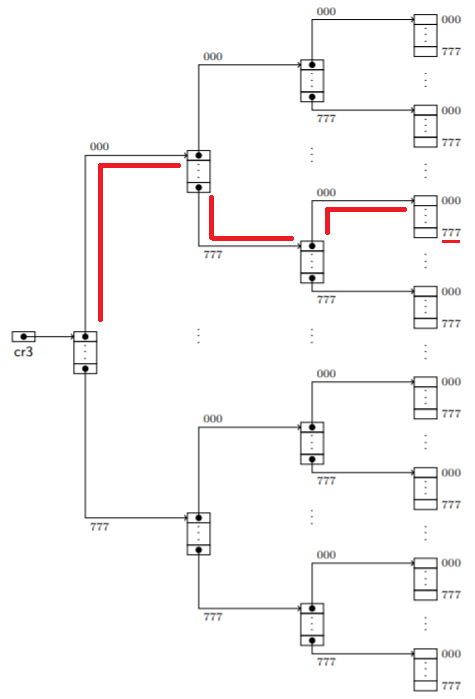
\includegraphics[scale=.8]{img/232.PNG}
	\end{center}
\end{framed} 
\clearpage 
\subsection{Esempio non vitale: creazione di un albero di traduzione in Assembler}
Proviamo a creare un albero di traduzione (non per usarlo, solo per capire come si ragiona all'avvio): vogliamo mappare .
Lo facciamo in Assembler.

\subsubsection{Codice Assembler}
\scriptsize
\begin{multicols}{2}
	\begin{verbatim}
		# vogliamo mappare i primi 8 MiB in se stessi
		#                          12
		# +--------------------------+-----------------+
		# |    n. frame              |          DAwdSWP|
		# +--------------------------+-----------------+
		
		.global setup_vm
		setup_vm:
		# 0 -> 0
		#  4   3   2   1   off
		# 000 000 000 000 xywz -> 000 000 000 000 xywz
		movq $tab3, tab4
		movb $0b00000111, tab4
		
		movq $tab2, tab3
		movb $0b00000111, tab3
		
		movabs $tab2, %rsi
		movabs $tab1_0, %rdi
		xor %rax, %rax
		
		.Loop0:
		mov %rdi, (%rsi)
		movb $0b00000111, (%rsi)
		xor %rcx, %rcx
		.Loop1:
		mov %rax, (%rdi, %rcx, 8)
		movb $0b00000111, (%rdi, %rcx, 8)
		add $0x1000, %rax
		cmp $511, %rcx
		jge .Lnext
		inc %rcx
		jmp .Loop1
		.Lnext:
		cmp $tab1_3, %rdi
		je .Lend
		add $4096, %rdi
		add $8, %rsi
		jmp .Loop0
		.Lend:	
		movabs $tab4, %rax
		mov %rax, %cr3
		
		ret
		
		.global a_page_fault
		a_page_fault:
		pop %rdi
		mov (%rsp), %rsi	
		mov %cr2, %rdx
		call c_page_fault
		hlt
		
		.data
		.global tab4, tab3, tab2, tab1_0, tab1_1, tab1_2, tab1_3, tab1_4
		.balign 4096
		tab4:
		.space 4096, 0
		tab3:
		.space 4096, 0
		tab2:
		.space 4096, 0
		tab1_0:
		.space 4096, 0
		tab1_1:
		.space 4096, 0
		tab1_2:
		.space 4096, 0
		tab1_3:
		.space 4096, 0
		tab2_3:
		.space 4096, 0
		tab1_4:
		.space 4096, 0
	\end{verbatim}
\end{multicols}
\small
\begin{itemize}
	\item \textbf{Allocazione dello spazio per l'albero}.
	\begin{itemize}
		\item Ci serve spazio per un albero di traduzione.
		\item La tabella non può essere allocata ovunque, deve essere posta a un indirizzo che è multiplo di 4096. Facciamo questo con la seguente istruzione
		\begin{verbatim}
			.balign 4096
		\end{verbatim}
		\item \textbf{Quante tabelle di livello quattro ci servono?} 
		
		Una, visto che abbiamo solo la radice dell'albero.
		\item \textbf{Quante tabelle di livello tre ci servono?} Sempre una. 
		\begin{itemize}
			\item Ogni riga copre $1\,\text{GB}$.
			\item Se moltiplico per il numero di righe otteniamo
			\[512 \cdot 1\,\text{GB} = 512\,\text{GB}\]
			per $8\,\text{MB}$ basta una sola tabella.
		\end{itemize}
		\item \textbf{Quante tabelle di livello due ci servono?} Sempre una. 
		\begin{itemize}
			\item Ogni riga copre $2\,\text{MB}$.
			\item Se moltiplico per il numero di righe ottengo
			\[2\,\text{MB} \cdot 512 = 1\,\text{GB}\]
			Anche in questo caso una sola tabella è più che sufficiente.
		\end{itemize}
		\item \textbf{Quante tabelle di livello $1$ ci servono?} Quattro.
		\begin{itemize}
			\item Ogni riga copre $4\,\text{KB}$
			\item Se moltiplico per il numero di righe ottengo
			\[4\,\text{KB} \cdot 512 = 2048\,\text{KB} \]
			Questa volta non ci basta una sola tabella, ne servono $4$.
		\end{itemize}
	\end{itemize}
	Codice con cui allochiamo lo spazio 
	\begin{multicols}{2}
		\begin{verbatim}
			.data
			.global tab4, tab3, tab2, tab1_0, 
			tab1_1, tab1_2, tab1_3, tab1_4
			.balign 4096
			tab4:
			.space 4096, 0
			tab3:
			.space 4096, 0
			tab2:
			.space 4096, 0
			tab1_0:
			.space 4096, 0
			tab1_1:
			.space 4096, 0
			tab1_2:
			.space 4096, 0
			tab1_3:
			.space 4096, 0
			tab2_3:
			.space 4096, 0
			tab1_4:
			.space 4096, 0
		\end{verbatim}
	\end{multicols}
	\item \textbf{Prepariamo l'albero}. 
	\begin{itemize}
		\item Dobbiamo pensare a come la MMU lo percorrerà (prende il numero di pagina, $0$, tralasciando l'offset). 
		\item Dobbiamo considerare, nei vari passaggi, la presenza di altre informazioni oltre al numero di frame: P, R/W, U/S, PCD, PWT, A, D. Alcuni di questi bit devono essere gestiti per forza, altrimenti non possiamo fare le nostre operazioni: settiamo i primi tre bit meno significativi (P, R/W, U/S). Lo facciamo aggiornando, di 64 bit, i 16 meno significativi
		\begin{verbatim}
			movb $0b00000111, tabX
		\end{verbatim}
		\item La prima riga di \emph{tab4} deve puntare \emph{tab3}, la prima riga di \emph{tab3} deve puntare a \emph{tab2}. 
		\begin{verbatim}
			movq $tab3, tab4
			movb $0b00000111, tab4
			
			movq $tab2, tab3
			movb $0b00000111, tab3
		\end{verbatim}
		\item Le righe di \emph{tab2} devono puntare alle tabelle di livello $1$. La cosa più conveniente è aggiornare le tabelle di livello $1$ attraverso dei cicli. 
		\begin{itemize}
			\item Le tabelle di livello $1$ sono una dopo l'altra, dunque non è necessario gestirle in modo distinto: si parte dalla prima riga della prima tabella di livello $1$ e si scorre tutto insieme.
			\item I parametri in ingresso sono due:
			\begin{itemize}
				\item registro RSI, indirizzo della tabella di livello $2$ \emph{tab2};
				\item registro RDI, indirizzo della prima riga della prima tabella di livello $1$.
			\end{itemize}
			\item Abbiamo due cicli annidati.
		\end{itemize}
		
	\end{itemize}
	\item \textbf{Aggiornamento di CR3}.
	
	Dopo aver riempito tutte le entrate di tutte le tabelle di livello $1$ possiamo mettere l'indirizzo dell'unica tabella di livello 4, \emph{tab4}, nel registro CR3. Da questo punto in poi non stiamo più utilizzando la traduzione preparata dal bootloader, ma la nostra.
	\begin{verbatim}
		movabs $tab4, %rax
		mov %rax, %cr3
	\end{verbatim}	
\end{itemize}
\normalsize 

\subsubsection{Codice C++} 
\small
\begin{verbatim}
	#include <libce.h>
	
	int var;
	
	extern "C" void setup_vm();
	extern "C" void a_page_fault();
	extern "C" natq tab4[], tab3[], tab2[], tab1_0[], tab1_1[], tab1_2[], tab1_3[], tab1_4[];
	extern "C" void c_page_fault(natq errore, natq rip, natq addr) {
		printf("errore %x, rip %x, addr %x\n", errore, rip, addr);
	}
	
	int main() {
		gate_init(14, a_page_fault);
		var = 1;
		printf("var = %d\n", var);
		pause();
		setup_vm();
		
		int *p = (int *)((natq)&var - 0x20f000 + 0x400000);
		printf("tab4[0] = %x\n", tab4[0]);
		printf("tab3[0] = %x\n", tab3[0]);
		printf("tab2[1] = %x\n", tab2[1]);
		printf("tab1_1[15] = %x\n", tab1_1[15]);
		
		printf("percorso alternativo:\n");
		printf("tab2[2] = %x\n", tab2[2]);
		printf("tab1_2[0] = %x\n", tab1_2[0]);
		*p = 2;
		printf("p %x, var = %d\n", p, var);
		printf("tab4[0] = %x\n", tab4[0]);
		printf("tab3[0] = %x\n", tab3[0]);
		printf("tab2[1] = %x\n", tab2[1]);
		printf("tab1_1[15] = %x\n", tab1_1[15]);
		
		printf("percorso alternativo:\n");
		printf("tab2[2] = %x\n", tab2[2]);
		printf("tab1_2[0] = %x\n", tab1_2[0]);
		
		pause();
	}
\end{verbatim}
\begin{itemize}
	\item \textbf{Eccezione \emph{page$\_$fault}}. 
	
	Immaginiamo di avere il seguente main
	\begin{verbatim} 
		int main() {
			var = 1;
			printf("var = %d\n", var);
			pause();
			setup_vm();
			pause();
		}			
	\end{verbatim} 
	Cosa succede dopo il secondo \emph{pause}? Si ha l'eccezione di tipo $14$ (\emph{page$\_$fault}), lanciata dalla MMU che non è riuscita a completare la traduzione. I motivi sono vari: incontra un bit $P=0$, scritture fallite perchè non è permessa la scrittura, o accessi ad aree di sistema in modalità utente...  Questa eccezione lascia in pila delle informazioni ulteriore: delle 4 quadword ci interessa quella in cima.
	\begin{itemize}
		\item Il bit meno significativo dice se l'errore è dovuto a una traduzione non valida ($0$) o a un errore di protezione ($1$).
		\item Il secondo bit meno significativo se l'eccezione è legata o meno a un'operazione di scrittura (si dice solo il tipo di operazione, non se era vietata la scrittura).
		\item Il terzo bit meno significativo segnala il livello di privilegio a cui si trovava il processore al momento dell'errore ($0$, sistema, $1$, utente). 
	\end{itemize} 
	Nel caso nostro abbiamo 
	
	\begin{center}
		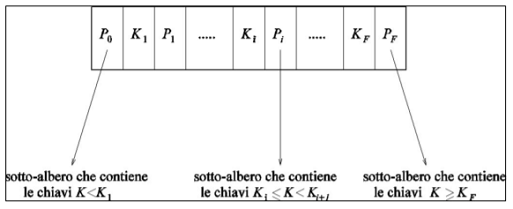
\includegraphics[scale=.8]{img/229.PNG}
	\end{center}
	L'errore è di traduzione, l'operazione era una scrittura in memoria
	\begin{verbatim}
		mov %edx, (%rax)
	\end{verbatim}
	\item \textbf{Registro CR2}.
	
	La MMU, quando non riesce a tradurre un indirizzo, scrive l'indirizzo che stava cercando di tradurre nel registro CR2.
	
	\item \textbf{Funzione da associare all'eccezione di tipo $14$}.
	
	Abbiamo scritto una routine da lanciare in caso di \emph{page$\_$fault}, come al solito divisa in due parti. La prima si trova nel codice Assembler visto prima e raccoglie i parametri in ingresso a partire dal contenuto della pila (ricordiamo che sono state poste delle informazioni in pila).
	\begin{itemize}
		\item RDI: quadword \emph{errore} (il codice identificativo dell'errore, che si trova in cima alla pila)
		\begin{verbatim}
			pop %rdi
		\end{verbatim} 
		\item RSI: quadword \emph{rip}, il rip dell'istruzione che il processore stava eseguendo quando si è manifestato il \emph{page fault}.
		\begin{verbatim}
			mov (%rsp), %rsi
		\end{verbatim}
		\item RDX: quadword \emph{addr}, contenuto del registro CR2 (l'indirizzo che la MMU non è riuscita a tradurre)
		\begin{verbatim}
			mov %cr2, %rdx
		\end{verbatim}
	\end{itemize}
	La seconda parte, in C++, richiede la stampa delle informazioni sull'eccezione
	\begin{verbatim}
		extern "C" void c_page_fault(natq errore, natq rip, natq addr) {
			printf("errore %x, rip %x, addr %x\n", errore, rip, addr);
		}
	\end{verbatim}
	Associo la funzione al tipo $14$ con la \emph{gate$\_$init}
	\begin{verbatim}
		gate_init(14, a_page_fault);
	\end{verbatim}
	L'output ottenuto è il seguente
	\begin{center}
		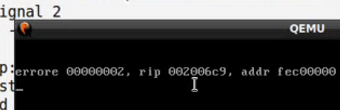
\includegraphics{img/231.PNG}
	\end{center}
	
	L'indirizzo a cui l'istruzione stava tentando di accedere è \emph{fec00000}. La traduzione di questo indirizzo virtuale non l'abbiamo creata: facciamolo!
	
	\item 	\textbf{Aggiunta di una nuova traduzione di indirizzo}.
	
	Traduciamolo in se stesso: la \emph{libce} pensava di utilizzare indirizzi fisici, la sua intenzione era di scrivere proprio a quell'indirizzo. Il codice Assembler viene aggiunto in \emph{setup$\_$vm}, dopo l'etichetta \emph{Lend}.
	\begin{multicols}{2}
		\begin{verbatim}
			# tab4
			# 0: -> tab3
			#       0: -> tab2
			#             0: tab1_0
			#             1: tab1_1
			#             2: tab1_2
			#             3: tab1_3
			#       3: -> tab2_3
			#             766: -> tab1_4
		\end{verbatim}
		\columnbreak
		\begin{verbatim}
			#	
			# fec00000 -> fec00000
			# 
			#   numero di pagina
			#
			# 000000000 000/000/011 111/110/110 000/000/000
			# 000       003         766         000
			#
			#
		\end{verbatim}
	\end{multicols}
	\begin{verbatim}	
		movl $tab2_3, tab3 + 8*3
		movb $0b00000111, tab3 + 8*3
		
		movl $tab1_4, tab2_3 + 0766 * 8 <--- 0766 interpretato in base 8
		movb $0b00000111, tab2_3 + 0766 * 8 <--- 0766 interpretato in base 8
		
		movl $0xfec00000, tab1_4
		movb $0b00001111, tab1_4
	\end{verbatim}
	\begin{itemize}
		\item Scomponendo l'indirizzo in ottave capiamo meglio come muoverci.
		\item Siamo in \emph{tab4}. Passiamo a \emph{tab3} attraverso la prima entrata dell'unica tabella.
		\item Siamo in \emph{tab3}: l'entrata che ci interessa è la terza, dunque abbiamo una nuova tabella da creare rispetto a prima (\emph{tab2$\_$3}).
		\item Nella tabella appena creata ci interessa la $502-$esima entrata. Attraverso questa si passa alla tabella \emph{tab1$\_$4} (ulteriore tabella in più).
		\item Le istruzioni mov per aggiornare il contenuto dell'albero le abbiamo già viste nella preparazione dell'albero. Si tenga solo conto che avendo l'APIC a quell'indirizzo conviene disattivare la cache: segue il settaggio del quarto bit meno significativo nelle varie \emph{movb}.
	\end{itemize}
	\item \textbf{Creazione di un nuovo indirizzo virtuale per la variabile \emph{var}}.
	
	Creiamo una variabile \emph{var} nel nostro programma.
	\begin{center}
		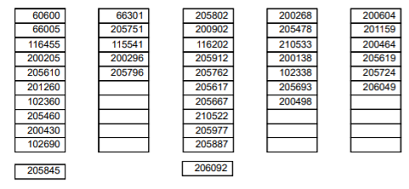
\includegraphics{img/230.PNG}
	\end{center}
	Siamo sicuri, per quello che abbiamo fatto prima, che già esista un indirizzo virtuale. Mappiamo un altro indirizzo virtuale, completamente diverso, nello stesso indirizzo fisico. Il codice Assembler viene aggiunto in \emph{setup$\_$vm}, dopo l'etichetta \emph{Lend}.
	\begin{verbatim}
		# 0x400-000 -> 0x20f-000
		#
		#  numero di pagina
		# 
		# 000000000 000000000 000000010 000000000
		# 000       000       002       000
		
		movl $0x20f000, tab1_2
		movb $0b0000111, tab1_2
	\end{verbatim}
	A livello di tabelle abbiamo già tutto, non ci serve fare altro. Entrata $0$ in \emph{tab4}, Ci interessano le seguenti entrate: entrata $0$ in \emph{tab3}, entrata $2$ in \emph{tab2}, entrata 0 in \emph{tab1$\_$2}. 
	
	A questo punto possiamo vedere, nel \emph{main}, l'utilizzo di questo nuovo indirizzo virtuale: la variabile \emph{var} viene modificata attraverso il puntatore \emph{p} (che contiene il nuovo indirizzo virtuale)
	\begin{verbatim}
		int *p = (int *)((natq)&var - 0x20f000 + 0x400000);
		*p = 2;
		printf("p %x, var = %d\n", p, var);
	\end{verbatim}
	
	\item \textbf{Modifica delle tabelle dell'albero in C++}.
	
	Possiamo notare come nel \emph{main} si recuperi diverse volte il contenuto delle tabelle dell'albero. Possiamo agire sulla tabella a partire dal C++, dopo aver definito il tipo. Nella lezione successiva è presente un esempio di scrittura (col cosiddetto \emph{Page Size Flag}).
\end{itemize}
\normalsize 

\section{Pagine di dimensione diversa (\emph{Page Size} flag)}
Abbiamo introdotto il trie, che ci offre il vantaggio di non avere sottoalberi se relativi indirizzi non sono utilizzati. Altra cosa utile è la possibilità di creare \textbf{pagine di dimensione diversa}.

\paragraph{Struttura indirizzo virtuale} Abbiamo:
\begin{itemize}
	\item 12 bit di offset (bit meno significativi);
	\item numero di pagina spezzato in quattro indici.
\end{itemize}
Più la pagina è grande, più è grande l'offset e piccolo il numero di pagina. 
\paragraph{Proposta} Se la dimensione delle pagine è variabile allora si potrebbe aumentarne la dimensione, arrivando a ridurre di $1$ i livelli dell'albero (velocità della traduzione - tre accessi invece di quattro - e minore spazio occupato dalla struttura dati). La cosa solitamente non succede perchè pagine di dimensioni più elevate possono comportare un maggiore spreco di memoria (si consideri che la pagina è unità di condivisione tra progetti, e di condivisione).

\paragraph{\emph{Page Size} flag} Nonostante questo l'albero ci permette di non dover decidere a priori la grandezza, possiamo decidere in modo flessibile. Questo perchè all'interno di ogni entrata abbiamo un flag \textbf{Page Size} (PS) che dica alla MMU che in questo percorso (supponiamo di settare il flag al livello $2$) la pagina è più grande (si indica che il percorso finisce lì, nell'esempio detto abbiamo una dimensione di $2\,\text{MB}$). Il set o meno di questo flag determina il numero di bit del numero di pagina all'interno dell'indirizzo virtuale.
\begin{itemize}
	\item \textbf{Vantaggio}: ci servono meno tabelle per fare la traduzione identità (quella dove indirizzi virtuali corrispondono a indirizzi fisici, nella parte di RAM riservata al sistema).
\end{itemize}

\subsection{Esempio di utilizzo del flag nell'ultimo esempio di esercizio}
Riprendiamo l'esercizio della scorsa lezione, abbiamo visto che possiamo leggere le tabelle dell'albero dal C++, dopo aver definito il tipo. Avevamo creato una traduzione (identità) solo fino a $8\,\text{MB}$, questo significa che se dichiaro qualcosa fuori da questa regione viene lanciata un'eccezione (per $P=0$).
\paragraph{Cosa vogliamo fare?} Adesso vogliamo creare una traduzione identità per altri $2\,\text{MB}$: senza le cose appena introdotte risulterebbe necessario introdurre una nuova tabella. Ci limitiamo a fare
\begin{verbatim}
	tab2[4] = 0x800000 | 0x87;
\end{verbatim}
settando il bit più significativo del byte di accesso, il bit PS. In questo modo diciamo ad MMU che la traduzione è già finita quando si arriva a questa entrata.


\section{Cache \emph{Translation Lookaside Buffer} (TLB)}
Dal punto di vista dell'hardware ci resta un'unica cosa. L'implementazione via trie è comoda ma presenta anche degli svantaggi: pensiamo al numero elevato di accessi (con questi alberi il numero di accessi moltiplica ogni volta\footnote{La cosa può avere grande impatto sul tempo di esecuzione di un programma: prelievo delle istruzioni, prelevo o scrittura degli operandi che si trovano in memoria...}). Anche accedere in cache ha un costo: il singolo accesso non occupa centinaia di clock, ma rispetto a prima abbiamo un numero maggiore di accessi in cache. 
\paragraph{Soluzione} La soluzione è la \emph{Translation Lookaside Buffer} (TLB), una cache dedicata alla MMU (una cache delle traduzioni, entro qua per non consultare il trie). 
\paragraph{Cache} Limitiamoci a parlare delle cache a $4\,\text{KB}$: la cache conterrà le entrate delle tabelle di livello $1$. La TBL è una letteralmente una cache a 8/16 vie. Lo schema interno è quasi del tutto identico a quello già visto.
\begin{center}
	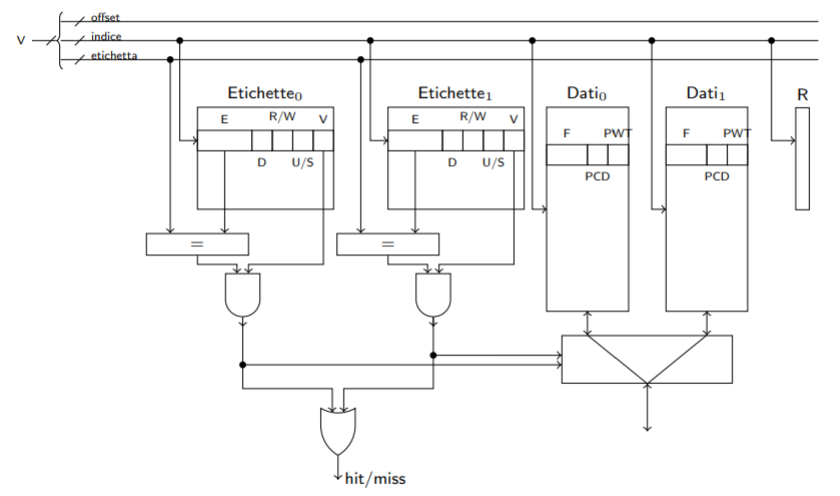
\includegraphics[scale=.8]{img/228.PNG}
\end{center}
Viene memorizzata l'associazione tra numero di pagina e numero di frame, oltre alle informazioni poste nel descrittore di pagina.

\paragraph{Osservazione su alcuni bit} 
\begin{itemize}
	\item Abbiamo detto che una pagina è riservata al sistema se tutti i bit U/S (uno per livello) sono settati. Che informazione metto nel TLB (1 bit) affinchè il controllo possa essere equivalente a quello fatto sul trie (4 bit))?
	La AND dei vari bit incontrati.
	\item Il bit A indica che c'è stato un accesso: non è riportato nel TLB perchè se l'entrata è presente in cache è logico che c'è stato un accesso.
	\item La cosa è più complessa col bit D: può accadere che su una data pagina ho inizialmente una lettura e poi una scrittura. In queste condizioni non ce ne accorgiamo passando dalla cache: $D$ rimane a zero nonostante la scrittura. {Risolviamo così: in caso di hit con operazione di scrittura e $D$ a zero non si concede immediatamente la scrittura (\emph{miss}), ma si ripercorre il trie}.   
	\item Il bit $P$ non è presente: se abbiamo riportato l'entrata nella cache significa che abbiamo trovato tutti i $P=1$.
	\item Se $V=0$ la riga non è significativa (è il bit già incontrato quando abbiamo spiegato la cache, non ha a che vedere con le entrate delle tabelle del trie)
\end{itemize}
\subsection{Riprendiamo l'esempio di esercizio} Abbiamo visto che è possibile modificare la variabile \emph{var} a partire da due indirizzi virtuali completamente diversi. Immaginiamo di avere il seguente main
\begin{verbatim}
	#include <libce.h>
	#include <vm.h> <----  novita'
	int var;
	
	extern "C" void setup_vm();
	extern "C" void a_page_fault();
	extern "C" natq tab4[], tab3[], tab2[], tab1_0[], tab1_1[], tab1_2[], tab1_3[], tab1_4[];
	extern "C" void c_page_fault(natq errore, natq rip, natq addr) {
		printf("errore %x, rip %x, addr %x\n", errore, rip, addr);
	}
	
	int main() {
		gate_init(14, a_page_fault);
		var = 1;
		prinft(var = %d\n", var);
		pause();
		setup_vm();
		int *p = (int*)((natq)&var - 0x20f000 + 0x400000);
		tab1_2[0] = 0x20f000 | 0x07;
		*p = 2;
		printf("var = %d\n", var)
		pause();
	}
\end{verbatim}
Se compiliamo vediamo di nuovo lo scrivere in \emph{var} attraverso un indirizzo virtuale alternativo. 
\begin{center}
	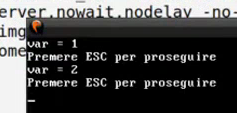
\includegraphics{img/233.PNG}
\end{center}
Aggiungiamo la seguente riga prima della scrittura in \emph{tab1$\_$2}.
\begin{verbatim}
	*p = 3;
\end{verbatim}
Stavolta \emph{var} non viene modificato, l'output da $1$.
\begin{center}
	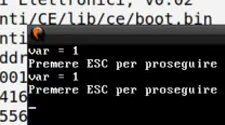
\includegraphics{img/234.PNG}
\end{center}
\paragraph{Come mai?} 
\begin{itemize}
	\item Inizialmente l'indirizzo \emph{0x400000} è mappato su se stesso. 
	\item Con la prima modifica
	\begin{verbatim}
		*p = 3
	\end{verbatim}
	agiamo sull'indirizzo fisico \emph{0x400000}. Segue che non modificheremo \emph{var} con questa istruzione.
	\item Con la seconda modifica, che avviene dopo l'aggiornamento della riga di \emph{tab1$\_$2}
	\begin{verbatim}
		*p = 2;
	\end{verbatim} La traduzione nel trie è ancora quella vecchia: abbiamo agito sempre su \emph{0x400000}, e non su \emph{var}.
	\item Non è la cache della memoria il problema, \textbf{ma la traduzione che ha usato la MMU}.
\end{itemize}
Questo problema è dovuto alla cache TLB. Il problema è il solito: mantenere la consistenza a seguito di modifiche. Quando modifico una traduzione il TLB quasi sicuramente non se ne accorge. Dobbiamo invalidarlo in modo esplicito! Possiamo farlo in due modi.
\begin{enumerate}
	\item \textbf{Istruzione mov con registro CR3 operando destinatario}
	\begin{verbatim}
		movq %rax, %cr3
	\end{verbatim}
	L'istruzione può potenzialmente alterare tutta la tabella di livello $4$, quindi tutte le informazioni contenute nel TLD non possono considerarsi più valide. 
	\item \textbf{Istruzione Assembler \emph{invlpg} (\emph{invalid page})}
	\begin{verbatim}
		invlpg operando_in_memoria
	\end{verbatim}
	L'istruzione permette di invalidare la traduzione relativa all'indirizzo passato come operando. La libreria \emph{libce},  \emph{vm.h}, offre una funzione già pronta per poter eseguire l'istruzione da C++: \textbf{invalida$\_$entrata$\_$TLB}.
	\begin{center}
		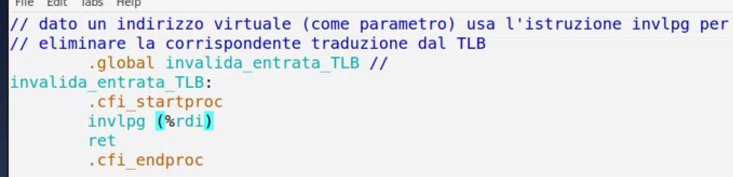
\includegraphics[scale=.8]{img/235.PNG}
	\end{center} 
\end{enumerate}
A questo punto torniamo sul \emph{main} e scriviamolo così
\begin{verbatim}
	int main() {
		gate_init(14, a_page_fault);
		var = 1;
		prinft(var = %d\n", var);
		pause();
		setup_vm();
		int *p = (int*)((natq)&var - 0x20f000 + 0x400000);
		
		*p = 3; <--- riga in piu'
		
		tab1_2[0] = 0x20f000 | 0x07;
		
		invalida_entrata_TLB(p); <--- riga in piu'
		
		*p = 2;
		printf("var = %d\n", var)
		pause();
	}
\end{verbatim}
L'output torna e la seconda modifica del contenuto puntato da \emph{p} ha agito su \emph{var}.